\documentclass[a4paper,12pt,oneside,openany,table,xcdraw]{article}

\usepackage{setspace}
\usepackage{multirow}
\usepackage{hyperref}
\usepackage{caption}
\usepackage{indentfirst}

\usepackage[brazilian]{babel}
\usepackage[utf8x]{inputenc}
\usepackage{amsmath, graphicx, enumerate}
\usepackage{float, verbatim}
\usepackage[colorinlistoftodos]{todonotes}
\usepackage{makeidx} % Para o sumário
\usepackage{geometry}

\geometry{a4paper, hmargin={3cm, 3cm}, vmargin={3cm, 2cm} }
\setlength{\parindent}{1.0cm}
\graphicspath{{img/}}
\captionsetup{font=small}

\begin{document}
\newcommand{\thedepartment}{Faculdade de Engenharia Elétrica}
\newcommand{\thecourse}{FEELT}
\newcommand{\thetitle}{FONTE LINEAR REGULADA + CIRCUITO AMPLIFICADOR}
\newcommand{\thetype}{Relatório da Disciplina de Eletrônica Analógica I}
\newcommand{\theproftitle}{Bacharel em Engenharia Elétrica}
\newcommand{\thestudent}{Ana Júlia Costa Santana \_ 
11811ETE003\\Lesly Viviane Montúfar Berrios \_ 
11811ETE001}
\newcommand{\theadvisor}{Prof. Daniel Pereira de Carvalho}
\newcommand{\thecity}{Uberlândia}

\thispagestyle{empty}\newcommand*{\themonth}{\ifthenelse{\the\month < 2}{Janeiro }
                  {\ifthenelse{\the\month < 3}{Fevereiro }
                  {\ifthenelse{\the\month < 4}{Março }
                  {\ifthenelse{\the\month < 5}{Abril }
                  {\ifthenelse{\the\month < 6}{Maio }
                  {\ifthenelse{\the\month < 7}{Junho }
                  {\ifthenelse{\the\month < 8}{Julho }
                  {\ifthenelse{\the\month < 9}{Agosto }
                  {\ifthenelse{\the\month < 10}{Setembro }
                  {\ifthenelse{\the\month < 11}{Outubro }
                  {\ifthenelse{\the\month < 12}{Novembro }{Dezembro }}}}}}}}}}}}
                  
\begin{titlepage}
\begin{center}

	\vspace{-0.5cm}

  \begin{figure}[hbt!]
		\begin{center}
		   
\includegraphics[width=2.8cm]{ufu-logo.png}
		\end{center}
	\end{figure}
 	%\vspace{-4cm}

%\begin{doublespacing}

  \Large{\textbf{Universidade Federal de Uberlândia}}\\
  \large{\thedepartment}\\
  \large{\thecourse}\\


\vspace{5.8cm}
  \par
  \large\textbf{\thetitle}
\vspace{5.8cm} 

%\end{doublespacing}
  \par
  \thetype\\
  por\\
  %\hspace{2cm}\large{}\\

\vspace{0.8cm}
\par
  \normalsize{\thestudent}\\ [2cm]
  \theadvisor

\par\vfill
  \thecity, \themonth / \the\year

\end{center}

\end{titlepage}

%% Comeca o documento !

\onehalfspacing
\tableofcontents % sumário
\newpage

\section{Introdução}
Na construcão e planejamento da primeira placa de impresso (\emph{PCB}) está a essência de qualquer curso da Faculdade de Engenharia Elétrica (FEELT), uma vez que, à despeito das dificuldades no entendimento da disciplica teórica, o planejamento e análise da forma de onda da gradezas de tensão e corrente demonstram e ilustram com lucidez cada processo intrínseco do circuito. Nesse sentido, o uso de simuladores, seja \emph{PROTEUS}, \emph{MULTSIM} ou qualquer outro, é ferramenta de imprescindível para a análise do qualquer circuito, e entendimento dos componentes necessários e melhor adaptáveis às exigências do projeto.

O projeto a ser destrinchado em cálculos e demostrações é retirado do material \emph{El Cheapo} \cite{cheapo} cujo título é \emph{Um realmente simples amplificador de potência} (do inglês, \emph{A Really Simple Power Amplifier}). Logo, é preciso planejar a elaboração de dois circuitos: a \emph{fonte de alimentação linear regulada} e o \emph{circuito amplificador}. Sabe-se que o projeto mencionado pode ser substituído em parte por um dispositivo menor (um amplificador operacional), contudo isso não é feito visto que o objetivo principal é o aprendizado dos componentes mais básicos da elétrica: reistores, capacitores, transistores e diodos. 

À respeito da \textbf{\textit{fonte de alimentação linear regulada}}, tratada na Seção \ref{fonte}, pode obter-se melhor experiência, seja na busca por componentes, assim como melhor envolvimento com ferramentas de simulação e elaboração de placas de circuito impresso. Sabendo-se 
 que trata-se de um dispositivo responsável por converter a tensão elétrica alternada em contínua, foi possível verificar experimentalmente as qualidades e resultados de um circuito retificador em ponte, além de fitros capacitivos e circuitos reguladores com diodos zener.

Já o \textbf{\textit{circuito amplificador}}, discutido na Seção \ref{amp}, pode e deve ser realizado com maior empenho, devido à experiência adquirida durante a realização da fonte. 

Na Seção \ref{fonte} são discutidos as características da fonte: componentes, memória de cálculo, simulação ...
A Seção \ref{amp} é subdividida de forma análoga ... 

\newpage
\section{Fonte de Alimentação Linear Regulada} \label{fonte}

\subsection{Componentes e orçamento} 
Com intuito de realizar primeiramente o circuito que alimentará o circuito amplificador, ou seja a fonte de alimentação, \emph{El Cheapo} sugere o esquemático da Figura \ref{fonte:esquematico}, o qual já foi adaptado em \cite{cheapo} para componentes mais modernos, por exemplo substituindo os transistores de germânio por outros de silício. Assim, extraí-se os componentes que estão dispostos na Tabela \ref{fonte:componentes}, na qual também verifica-se o orçamento total para esta etapa, nas lojas de eletrônicos de Uberlândia, sendo visitadas Mundo Eletrônico, Ponto Eletrônico, Rádio Peças Uberlândia e Ponto Eletrônico para a aquisição de todos os componentes necessários.
\vspace{0.2cm}

\begin{figure}[H]
\centering
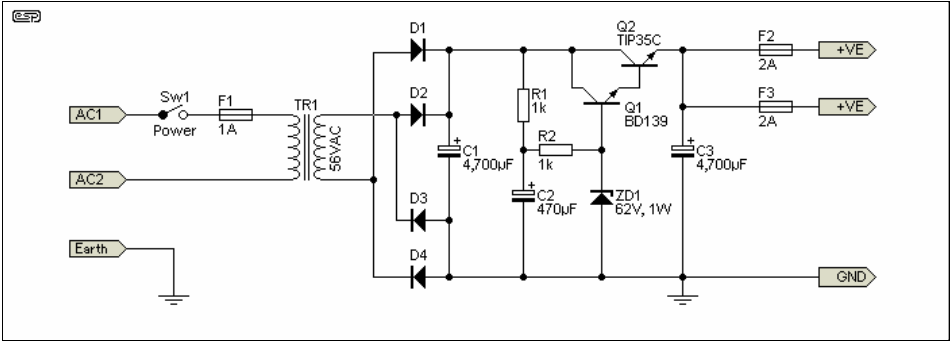
\includegraphics[width=15cm]{fonte-esquematico}
\caption{Esquemático \emph{El Cheapo} do circuito alimentador \cite{cheapo}.}
\label{fonte:esquematico}
\end{figure}
\vspace{0.4cm}

A escolha dos componentes da Tabela \ref{fonte:componentes} também exige análise do circuito mediante um simulador ou análise do circuito, seja por malhas ou nodal, visto que devem ser projetados para uma tensão suficientemente alta. Para todo componente, existe essa limitação intrínseca do material, por exemplo a ponte retificadora escolhida foi a GBJ606, dado que suporta uma corrente máxima de 6A e tensão máxima de 600V.

%\item Existe de especificação de tensão máxima no datasheet, para as pontes retificadoras?
%\item O resistor de descarga só é necessário para fonte sem carga, entao retiro do orcamento? (Mas preciso dos resistores de for querer uma fonte independente, certo? Para mim, que eu possa regular a tensao de saida e corrente) 


\begin{table}[H]
\def\arraystretch{1.28}
\centering
\caption{Componentes e orçamento da fonte.}
\label{fonte:componentes}
\resizebox{\textwidth}{!}{%
\begin{tabular}{cc|c|c|c}
\hline
\multicolumn{1}{|c|}{\textbf{Componente}}           & \textbf{Especificação} & \textbf{Quantidade} & \textbf{Preço (R\$)}         & \multicolumn{1}{c|}{\textbf{Descrição}}    \\ \hline
\multicolumn{1}{|c|}{\multirow{2}{*}{Capacitores}}  & $4700 \mu F - 100V$           & 2                   & 10+25 = 35                   & \multicolumn{1}{c|}{C1, C3}                \\ \cline{2-5} 
\multicolumn{1}{|c|}{}                              & $470 \mu F - 100V$            & 1                   & 9,50 (2,00)                  & \multicolumn{1}{c|}{C2}                    \\ \hline
\multicolumn{1}{|c|}{\multirow{2}{*}{Resistores}}   & $1k \Omega$            & 2                   & $2\times 0,06 = 0,12$        & \multicolumn{1}{c|}{R1, R2}                \\ \cline{2-5} 
\multicolumn{1}{|c|}{}                              & $1k8 \Omega$ - 5W      & 2                   & $2\times 2,42 = 4,84$        & \multicolumn{1}{c|}{Descarga do capacitor} \\ \hline
\multicolumn{1}{|c|}{Ponte Retificadora}            & 6A                     & 1                   & 7,15                         & \multicolumn{1}{c|}{Havia a GBJ606}        \\ \hline
\multicolumn{1}{|c|}{\multirow{2}{*}{Transistores}} & BD139                  & 1                   & 0,85                         & \multicolumn{1}{c|}{Q1}                    \\ \cline{2-5} 
\multicolumn{1}{|c|}{}                              & TIP35C                 & 1                   & 5,85                         & \multicolumn{1}{c|}{Q2}                    \\ \hline
\multicolumn{1}{|c|}{Fusível}                       & 4A                     & 1                   & 0,30                         & \multicolumn{1}{c|}{FUS}                   \\ \hline
\multicolumn{1}{|c|}{Borne Painel}                  & 5A                     & 4                   & 	5,25	  & \multicolumn{1}{c|}{Só havia de 20A}       \\ \hline
\multicolumn{1}{|c|}{Placa de fenolite}             & $10\times 15cm$        & 1                   & 6,80                         & \multicolumn{1}{c|}{Tamanho adequado}      \\ \hline
                                                    &                        & \textbf{Total:}     & R\$ 75,66                    &                                            \\ \cline{3-4}
\end{tabular}%
}
\end{table}

\vspace{0.2cm}
\subsection{Memória de cálculo} % com simulações!
Cada componente possui uma função no circuito, que pode ser analisada a nível de tensão e corrente. Espera-se um sinal contínuo na saída, com o qual poderá conectar-se a carga, ou seja o circuito amplificador de $8 \Omega$.

\subsubsection{Retificação}
Esta etapa transforma a tensão alternada em uma tensão contínua pulsante, e é realizada principalmente pela ponte retificadora. a ponte escolhida foi uma de 6A, 100 V que atende aos parâmetros do circuito montado.

%%%%%%%%%%%% simulaçao sem carga como fazer?

\subsubsection{Filtragem}
Transforma a tensão contínua pulsante em uma tensão contínua quase perfeita. Mas essa tensão contínua apresenta, quando a fonte é ligada a uma carga, uma oscilação chamada Tensão de Ripple. Essa etapa é realizada pelos capacitores encontrados eno circuito que devido a sua composição, ao sofrer o processo de carga e descarga diminuem a oscilação da tensão já que a tensão fornecida ao circuito agora nos momentos de pulso é suprida pela descarga do capacitor. Porém como abprdado anteriormente, resta ainda o riplle e para eliminar esse fator incômodo existe ainda outra etapa...

\subsubsection{Regulação}
Após a retificação e a filtragem,ocorre a etapa de regulação, com o objetivo de eliminar definitivamente a tensão de oscilação, mesmo com uma carga variável. O diodo utilizado, conta com uma tensão Zener nominal de 62 V para uma corrente de teste de 4 mA.

O comportamento do zener é observado para dois processos, a regulação de linha, que mostra acapacidade da fonte de manter a tensão de saída diante de variações na tensão de entrada.

Se a tensão de entrada aumenta muito, ao invés de ter todo esse acréscimo em cima da carga, o diodo Zener, regula esse valor de tensão, por meio da sua característica de operação em ruptura reversa. Isso é bem observado na corrente, que sofre maiores alterações para que a tensão se mantenha constante.Para o processo inverso, com um descréscimo na tensão de entrada, um processo análogo. As variações na tensão de entrada, são direcioandas ao resistor limitador, mostrando serem válidas as equações abaixo.

\begin{equation}
I_{S}  = I_{Z} +I_{R}  
\end{equation}
\begin{equation}
V_{S}  = V_{in} - V_{Z}
\end{equation}

Existe ainda a  regulação de carga, que mostra a capacidade da fonte de manter uma tensão de sída constante diante de variações na corrente de carga. Que depende da potência requerida pela carga.
\begin{equation}
I_{S}  =\frac{ V_{in} - V_{Z}  }{R_{S}}
\end{equation}
Logo, para toda a avariação na corrente de carga é compensada por uma variação oposta na corrente através do diodod Zener, mantendo a tensão constante.


\subsubsection{Resistor para descarga do capacitor} \label{descarga}
Para segurança do circuito,e daqueles que forem manejá-lo, resistores foram acrescentados em paralelo com os capacitores, para que, ao efetuar o desligamento da placa os capacitores pudessem ser descarregados em segurança.
Para projetar a resistência necessária nos capacitores, as equações conhecidas para descarga num capacitor foram aplicadas.

\begin{equation}
t= RC \cdot ln\bigg( 1 - \frac{V_{C}}{V_{in}} \bigg) 
\end{equation}

Considerndo os capacitores de 4700uF e um tempo de descarga de 10 s, para uma tensão média entre os dois capacitores, $V_{C}$ de $64,85 V$ (de acordo com simulação) e $V_{in}$ de 80 $V_{pp}$, a resitência mínima necessária é de $1,3 k\Omega$, para suprir esses requisitos mínimos, foi utilizado um reistor de $1,8 k\Omega$ de $5W$. 


\subsection{Finalização e considerações sobre a PCB}

\subsubsection{Espessura da linha}
Ao projetar a plca de circuito impresso. Um cuidado maior com relação as trilhas precisa ser tomado, para que não haja problemas quanto a passagem de corrente, e para otimizar a dissipção do calor na placa. 
Para escolher uma espessura de linha que cumprisse tais propósitos, utilizamos o equacionamento de acordo com a norma IPC-2221, que através de sua curva define as constantes k, b e c que são utilizadas no cálculo da espessura da trilha mais adequada.
Iniciando pelo cálculo da área temos:
\begin{equation}
A [\mathit{th^{2}}] = \Bigg(\dfrac{I}{k \cdot (Temp-Rise [deg. C])^{b}}\Bigg)^{\frac{1}{c}}
 \end{equation}
 \vspace{0.3cm}

E em sequência a largura é dada:

\begin{equation}
L [\mathit{th}] = \dfrac{A}{Espessura [oz] \cdot 1,378}
 \end{equation}
\vspace{0.3cm}

Considerando  $k = 0,048$, $b = 0,44$, $c = 0,725$ e a placa de fenolite de \emph{1 OZ}, e uma variação de temperatura de aproximadamente $10^{\circ}C$, descobriu-se um valor para a espessura das linhas de aproximadamente $90 th$, o qual foi utilizado na maioria das trilhas do projeto.

\vspace{0.2cm}
\subsubsection{Projeto final no \emph{PROTEUS}}
Utilizando todos os conceitos já descritos foi possível organizar os componentes em uma placa de cirucito impresso, utilizando o software \emph{PROTEUS}.
\begin{figure}[H]
\centering
\captionsetup{font=scriptsize}
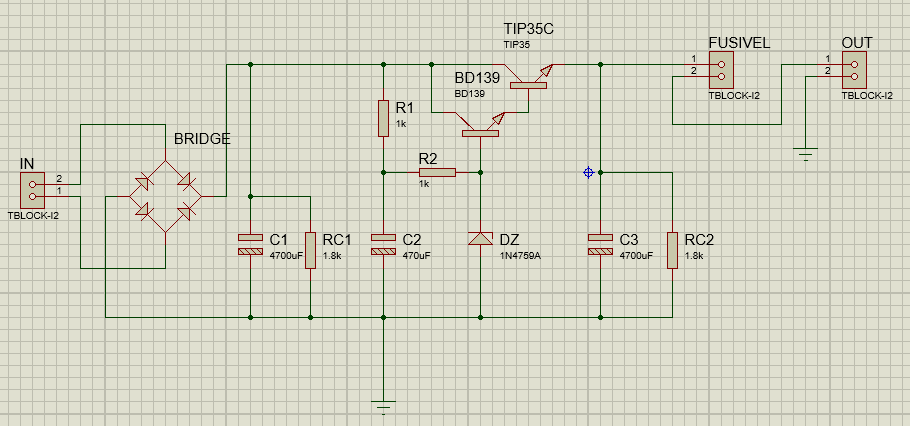
\includegraphics[width=15cm]{isis}
\caption{Projeto ISIS da fonte.}
\label{isis}
\end{figure}

\begin{figure}[H]
\centering
\captionsetup{font=scriptsize}
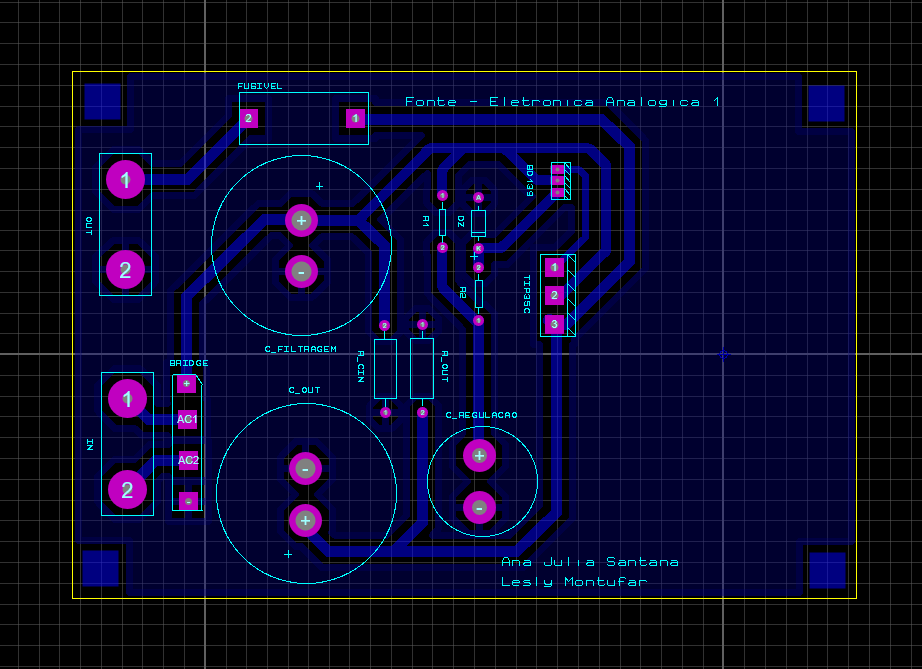
\includegraphics[width=15cm]{ares}
\caption{Projeto ARES da fonte.}
\label{ares}
\end{figure}

\begin{figure}[H]
\centering
\captionsetup{font=scriptsize}
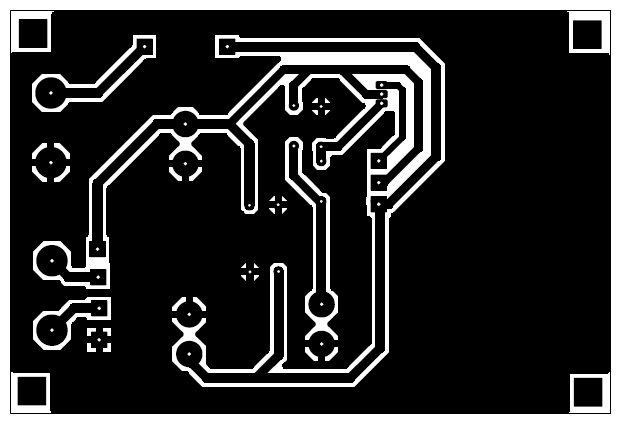
\includegraphics[width=15cm]{bottom}
\caption{Parte inferior do placa.}
\label{bottom}
\end{figure}

\begin{figure}[H]
\centering
\captionsetup{font=scriptsize}
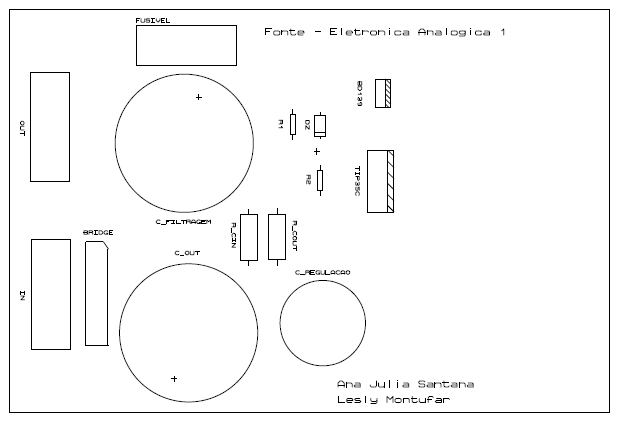
\includegraphics[width=15cm]{top}
\caption{Parte superior da placa.}
\label{top}
\end{figure}

\subsection{Testes e ensaios} %%%%%%%%%%%%%%%%%%%%%%%%%%%%%%%%%%%%%%%%%%%%%%%%% fazer!
\subsubsection{Regulação de linha}

\subsubsection{Regulação de carga}


\newpage
\section{Circuito amplificador} \label{amp}
\subsection{Componentes e orçamento} 
O esquemático \emph{El Cheapo}, apresentado na Figura \ref{amp:esquematico}, possui alguns dispositivos que são obsoletos hoje, por exemplo os trasistores de germânio, os quais podem ser equivalentemente substituidos pelos componentes descritos na Tabela \ref{amp:componentes}. 
\vspace{0.2cm}

\begin{figure}[H]
\centering
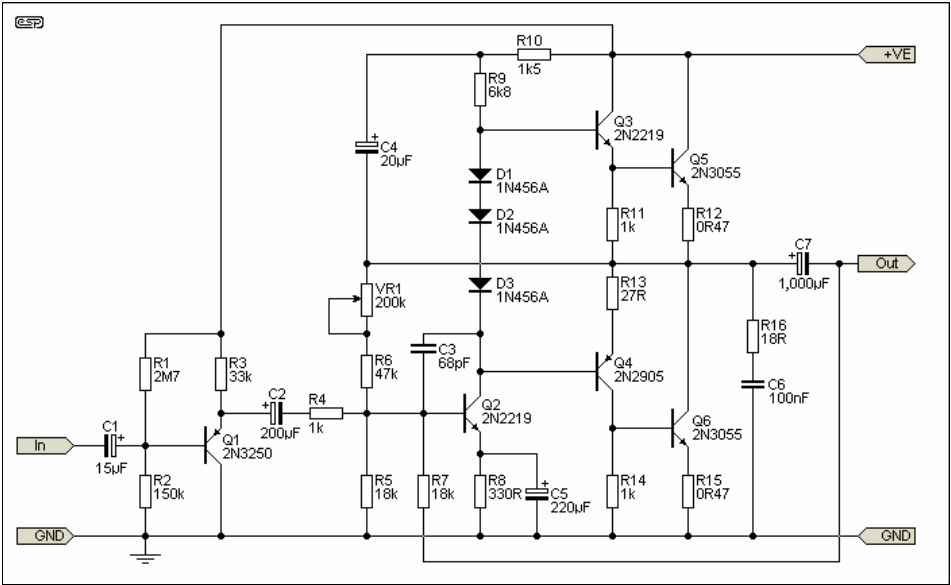
\includegraphics[width=15cm]{amp-esquematico}
\caption{Esquemático \emph{El Cheapo} do circuito amplificador \cite{cheapo}.}
\label{amp:esquematico}
\end{figure}

\vspace{0.4cm}
Dos componentes da Tabela \ref{amp:componentes}, extraídos do esquemático da Figura \ref{amp:esquematico}, ainda são possíveis mudanças para o aprimoramento dos mecanismo do circuito. O capacitor $C7$* por exemplo poderia ter aumento de capacitância para $4700 \mu F$, com o intuito de suprir o amortecimento insuficiente do arranjo de capacitores. %%%%%%%%%%%%%%%%%%%%%%%%%%%%%%%%%%%%%%%%%%%%%%%%%%%%%%%%%%%%%%%%%%%%%%%%%%%%%%%%%%%%%%%%%%%%%%%%%%%%%%%%%%%%%%%%%%%%%%%%%%%%%%%%%%%%%%%%%%%%%%%%%%%%%%%%%%%%%%%%%%%% justificar melhor, entender com graficos e simulacoes
Ademais, é importante ressaltar que os diodos (D1, D2 e D3) devem estar em contato com o dissipador, uma vez que da simulação se terá uma tensão em torno de 4 vezes a tensão de pico da fonte. %%%%%%%%%%%%%%%%%%%%%%%%%%%%%%%%%%%%%%%%%%%%%%%%%%%%%%%%%%%%%%%%%%%%%%%%%%%%%%%%%%%%%%%%%%%%%%%%%%%%%%%%%%%%%%%%%%%%%%%%%%%% explicar falando da tensao, eu acho, por meio de simulacao

\begin{table}[H] \scriptsize
\def\arraystretch{1.28}
\centering
\caption{Componentes e orçamento do circuito amplificador.}
\label{amp:componentes}
\resizebox{\textwidth}{!}{%
\begin{tabular}{cc|c|c|cc}
\hline
\multicolumn{1}{|c|}{\textbf{Componente}}           & \textbf{Especificação} & \textbf{Quantidade} & \textbf{Preço} & \multicolumn{1}{c|}{\textbf{Descrição}} & \multicolumn{1}{c|}{\textbf{Observações}}          \\ \hline
\multicolumn{1}{|c|}{\multirow{7}{*}{Capacitores}}  & $15 \mu F$             & 1                   &                & \multicolumn{1}{c|}{C1}                 & \multicolumn{1}{c|}{}                              \\ \cline{2-6} 
\multicolumn{1}{|c|}{}                              & $200 \mu F$            & 1                   & 5,00           & \multicolumn{1}{c|}{C2}                 & \multicolumn{1}{c|}{}                              \\ \cline{2-6} 
\multicolumn{1}{|c|}{}                              & $68 p F$               & 1                   & 0,50           & \multicolumn{1}{c|}{C3}                 & \multicolumn{1}{c|}{50V cerâmico}                           \\ \cline{2-6} 
\multicolumn{1}{|c|}{}                              & $20 \mu F$             & 1                   & 0,76           & \multicolumn{1}{c|}{C4}                 & \multicolumn{1}{c|}{22UF 100V}                     \\ \cline{2-6} 
\multicolumn{1}{|c|}{}                              & $220 \mu F$            & 1                   & 6,20           & \multicolumn{1}{c|}{C5}                 & \multicolumn{1}{c|}{220MF 100V (6,20) 220V (5,00)} \\ \cline{2-6} 
\multicolumn{1}{|c|}{}                              & $100 nF$               & 1                   & 0,42           & \multicolumn{1}{c|}{C6}                 & \multicolumn{1}{c|}{100k 50V cerâmico}             \\ \cline{2-6} 
\multicolumn{1}{|c|}{}                              & $1000 \mu F$           & 1                   & 1,20           & \multicolumn{1}{c|}{C7*}                & \multicolumn{1}{c|}{4700MF 63V(15,50)/1000MF 25V}  \\ \hline
\multicolumn{1}{|c|}{\multirow{12}{*}{Resistores}}  & $2M7 \Omega$           & 1                   &                & \multicolumn{1}{c|}{R1}                 & \multicolumn{1}{c|}{}                              \\ \cline{2-6} 
\multicolumn{1}{|c|}{}                              & $150k \Omega$          & 1                   & 0,10           & \multicolumn{1}{c|}{R2}                 & \multicolumn{1}{c|}{1/8W}                          \\ \cline{2-6} 
\multicolumn{1}{|c|}{}                              & $33k \Omega$           & 1                   & 0,10           & \multicolumn{1}{c|}{R3}                 & \multicolumn{1}{c|}{1/8W}                          \\ \cline{2-6} 
\multicolumn{1}{|c|}{}                              & $1k \Omega$            & 3                   & 0,15           & \multicolumn{1}{c|}{R4, R11, R14}       & \multicolumn{1}{c|}{}                              \\ \cline{2-6} 
\multicolumn{1}{|c|}{}                              & $18k \Omega$           & 2                   & 0,16           & \multicolumn{1}{c|}{R5, R7}             & \multicolumn{1}{c|}{1/8W}                          \\ \cline{2-6} 
\multicolumn{1}{|c|}{}                              & $47k \Omega$           & 1                   & 0,10           & \multicolumn{1}{c|}{R6}                 & \multicolumn{1}{c|}{1/8W}                          \\ \cline{2-6} 
\multicolumn{1}{|c|}{}                              & $330R \Omega$          & 1                   & 0,10           & \multicolumn{1}{c|}{R8}                 & \multicolumn{1}{c|}{1/8W}                          \\ \cline{2-6} 
\multicolumn{1}{|c|}{}                              & $6k8 \Omega$           & 1                   & 0,10           & \multicolumn{1}{c|}{R9}                 & \multicolumn{1}{c|}{1/8W}                          \\ \cline{2-6} 
\multicolumn{1}{|c|}{}                              & $1k5 \Omega$           & 1                   & 0,10           & \multicolumn{1}{c|}{R10}                & \multicolumn{1}{c|}{1/8W}                          \\ \cline{2-6} 
\multicolumn{1}{|c|}{}                              & $0R47 \Omega$          & 2                   & 0,20           & \multicolumn{1}{c|}{R12, R15}           & \multicolumn{1}{c|}{1/8W}                          \\ \cline{2-6} 
\multicolumn{1}{|c|}{}                              & $27R \Omega$           & 1                   & 0,10           & \multicolumn{1}{c|}{R13}                & \multicolumn{1}{c|}{1/8W}                          \\ \cline{2-6} 
\multicolumn{1}{|c|}{}                              & $18R \Omega$           & 1                   & 0,05           & \multicolumn{1}{c|}{R16}                & \multicolumn{1}{c|}{1/8W}                          \\ \hline
\multicolumn{1}{|c|}{Diodos}                        & 1N456A                 & 3                   &                & \multicolumn{1}{c|}{D1, D2, D3.}        & \multicolumn{1}{c|}{}                              \\ \hline
\multicolumn{1}{|c|}{\multirow{4}{*}{Transistores}} & BC559                  & 1                   & 0,93           & \multicolumn{1}{c|}{Q1}                 & \multicolumn{1}{c|}{}                              \\ \cline{2-6} 
\multicolumn{1}{|c|}{}                              & BD139                  & 2                   & 5,40           & \multicolumn{1}{c|}{Q2, Q3}             & \multicolumn{1}{c|}{}                              \\ \cline{2-6} 
\multicolumn{1}{|c|}{}                              & BD140                  & 1                   & 1,68           & \multicolumn{1}{c|}{Q4}                 & \multicolumn{1}{c|}{}                              \\ \cline{2-6} 
\multicolumn{1}{|c|}{}                              & 2N3055 (TIP35C)        & 2                   & 11,82           & \multicolumn{1}{c|}{Q5, Q6}             & \multicolumn{1}{c|}{}                              \\ \hline
\multicolumn{1}{|c|}{Potenciômetro}                 & 200k                   & 1                   &  2,75              & \multicolumn{1}{c|}{VR1}                & \multicolumn{1}{c|}{}                              \\ \hline
\multicolumn{1}{l}{}                                &                        & Total:              & R\$  35,17     &                                         &                                                    \\ \cline{3-4}
\end{tabular}%
}
\end{table}

\newpage
\section{Finalização do projeto: Fonte + Circuito amplificador}
%%%% ideia: chave liga e desliga e caixinha

\newpage
\section{Conclusões}
%%%% ideia: chave liga e desliga e caixinha



\begin{comment}
\section{Circuito esquemático}

\subsection{Componentes}
\begin{enumerate}[1 -]
    \item \textbf{\emph{Ponte retificadora:}} Optou-se pela ponte retificadora GBJ606 \cite{GBJ606}, pois possui corrente máxima de 6A.
    \item \textbf{\emph{Capacitores:}} De acordo com a disponbilidade de capacitores nos principais pontos de venda de eletrônicos em Uberlândia, conseguiu-se dois capacitores de $4700\mu F$ - 100V e um capacitor de $470\mu F$ - 200V.
    \item \textbf{\emph{Resistores:}} Foram utilizados dois resistores de 1k para regulação e dois de 1.8k - 5W para descarga do capacitor (não foi encontrado de imediato, para a venda, o resistor de potencia adequado).
    \item \textbf{\emph{Diodo Zener:}} Utlizado na regulação foi optado pelo diodo zener 1N4759.
    \item \textbf{\emph{Transistores:}} Foram utilizados TIP35C (100V) \cite{TIP35} e BD139 \cite{BD139}.
    \item \textbf{\emph{Fusível:}} Foi deduzido pela simulação que seria adequado um fusível de 4A ou até 2A nessa fase inicial, uma vez que já que não há carga conectada a corrente é nula, pois não é exigida pela carga. 
\end{enumerate}


\section{Simulação}
Para a realização de cada etapa foi essencial a verificação de tensão e correntes máximas sobre os componentes a fim de evitar um curto-circuito.
Por exemplo, antes de realizar a compra dos capacitores foi necessária a verificação da tensão máxima que este deveria suportar, a qual observa-se na Figura \ref{sim2}. Assim, verificou-se que seriam necessários capacitores que suportassem 80V ou mais, porém devido à disponibilidade escassa de capacitores na medida à risca, optou-se por dois capacitores 100V ($4700\mu F$) e um, 200V ($470\mu F$). Note que, já que a fonte não possui carga conectada, foi suposota uma carga de valor baixo de $0,5 \Omega$.

\begin{figure}[H]
\centering
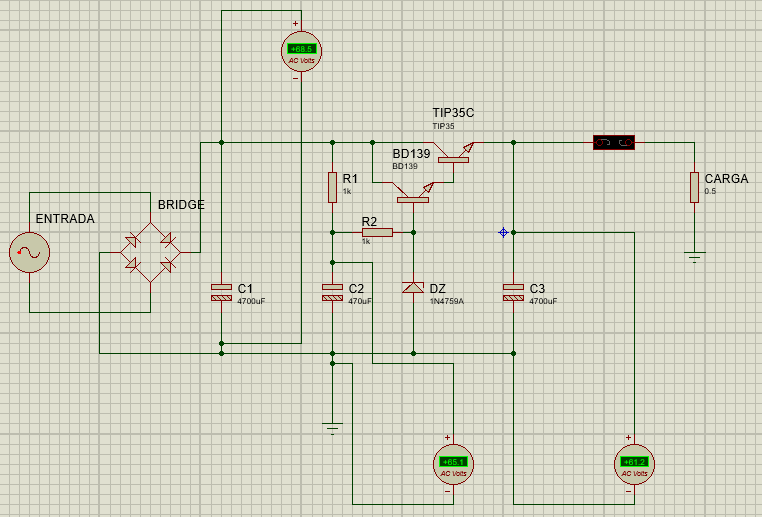
\includegraphics[width=15cm]{sim2}
\caption{Tensões máximas sobre os capacitores.}
\label{sim2}
\end{figure}

Agora pensando numa carga de $8 \Omega$ (do amplificador a ser conectado) obtem-se maiores tensões, e a partir dessa estimativa é possível projetar o fusível a ser utilizado na saída, pois, conforme à Figura \ref{com-carga}, espera-se uma corrente em torno de $5,68\ A$.

\begin{figure}[H]
\centering
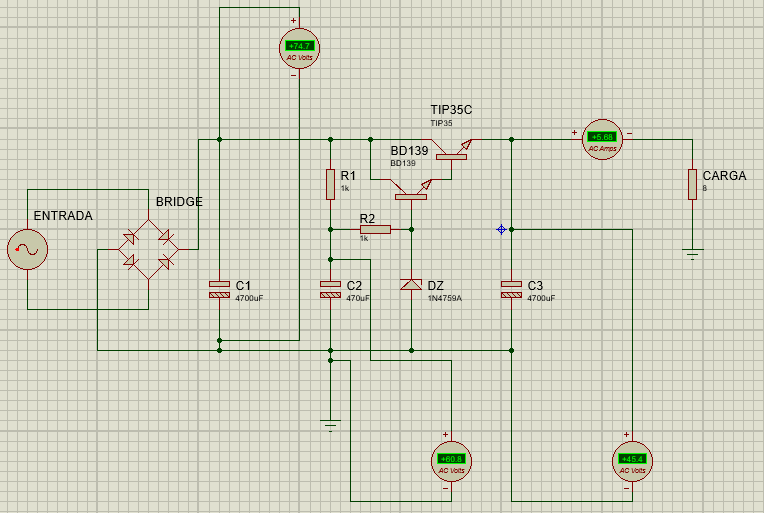
\includegraphics[width=15cm]{com-carga}
\caption{Tensões e correntes para uma carga de $8\Omega$.}
\label{com-carga}
\end{figure}

Ainda é interessante projetar resistores de descarga para o capacitor, uma vez que, sem carga conectada, é medida de segurança descarregar o capacitor.
Para isso, foi pensado num valor de resistência que conferisse pequeno tempo de descarga para capacitor. Assim, um resistor por exemplo de $1,8k\Omega$ possui tempo de descarga de aproximadamente $40s$, conforme os cálculos explicitados na seção \ref{descarga}. Dessa maneira, a simulação de um circuito com essas características resulta na Figura \ref{sim3}. Percebe-se que os resistores cumprem sua função de descarga do capacitor e desviam pequeno valor de corrente, de aproximadamente $25mA$. Para o capacitor de $470\mu F$ não é necessário um resistor de descarga, já que descarrega relativamente rápido, devido à sua baixa capacitância.

\begin{figure}[H]
\centering
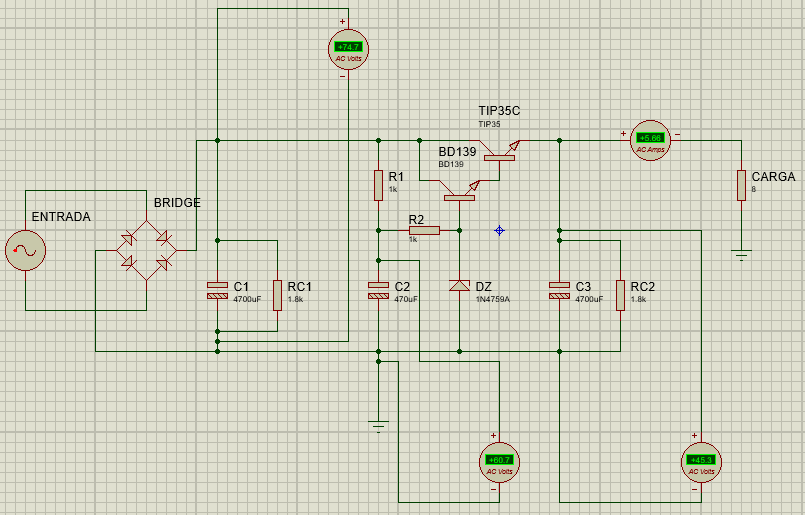
\includegraphics[width=15cm]{sim3}
\caption{Tensões e correntes com resistores de descarga de capacitor conectados.}
\label{sim3}
\end{figure}

\newpage
\section{Funcionamento do circuito}
A tensão de entrada é primeiramente rebaixada de $220V/127V$ para $56V$ com auxílio do regulador de tensão (também chamado de \emph{varivolt}). Assim, obter-se-á uma tensão senoidal de menor amplitude que ainda será convertida em contínua com intuito de ser utilizada para alimentar o amplificador.
\end{comment}


\newpage
\begin{thebibliography}{9} 
\bibitem{cheapo}
    Rod Elliott,
    “El Cheapo - A Really Simple Power Amplifier”, ESP, Elliott Sound Products, 2005.
 Disponível em:
 \url{https://sound-au.com/project12a.htm}. Acesso em: out. 2019.
 
 \bibitem{espess}
    Brooks Doug,Graves Dave,
    "Current Carrying Capacity of Vias"
 Disponível em: 
 \url{https://www.ultracad.com/articles/viacurrents.pdf}. Acesso em: out. 2019.
 
 \bibitem{res}
    Soares Camila,
 "Dedução das equações de carga e descarga dos capacitores utilizando equações diferenciais de primeira ordem". 
  Disponível em: 
% \url{https://camilasoares.wordpress.com/2009/04/07/deducao-das-equacoes-de-carga-e-descarga-dos-capacitores-utilizando-equacoes-diferenciais-de-primeira-ordem/}.
https://camilasoares.wordpress.com/2009/04/07/deducao-das-equacoes-de-carga-e-descarga-dos-capacitores-utilizando-equacoes-diferenciais-de-primeira-ordem/ 
Acesso em: out. 2019.
 
 \bibitem{comp}
    Petry Clovis Antonio,
 "D. PROJETO DE PLACAS DE CIRCUITO
IMPRESSO - BÁSICO "
  Disponível em: 
 \url{http://www.professorpetry.com.br/Bases_Dados/Apostilas_Tutoriais/Projeto_PCI_Charles.pdf}. Acesso em: out. 2019.
 
 % DATASHEETS
 
 \bibitem{GBJ606} % ponte retificadora
        “6.0A GLASS PASSIVATED BRIDGE RECTIFIER”, DIODES INCORPORATED.
 Disponível em:
 \url{https://www.diodes.com/assets/Datasheets/ds21216.pdf}. Acesso em: out. 2019.
 
  \bibitem{BD139} % transistor
    “BD135/137/139”, FAIRCHILD SEMICONDUCTOR.
 Disponível em:
 \url{http://www.redrok.com/NPN_BD135_45V_1.5A_12.5W_Hfe40_TO-126.pdf}. Acesso em: out. 2019.
 
 \bibitem{TIP35} % transistor
    “Silicon NPN Power Transistors TIP35/35A/35B/35C ”, SavantIC Semiconductor. 
 Disponível em:
 \url{https://pdf1.alldatasheet.com/datasheet-pdf/view/269985/SAVANTIC/TIP35.html}. Acesso em: out. 2019.
 


\end{thebibliography}
\end{document}
